% Suggested insertion after the Flat/Graph definitions in Initial Implementation.
\paragraph{Example of evidence organization.}
Figure~\ref{fig:worldstate-170} illustrates the representation on item 170.
The extractor identifies a bottle, a tray, and a gripper across two views,
assigning observations to shared entity identifiers. For example, observations
$o_1$ and $o_4$ describe entity $e_1$ in images 1 and 2; Graph places both
under the bottle node, whereas Flat lists entity and observation statements
separately. The cross-view flags are model-generated, with medium uncertainty
and no parser repairs. Graph answers correctly while Raw and Flat do not.
This outcome-selected example demonstrates the implemented grouping, but
does not establish that grouping caused the correction: the inventory contains
no spatial-relation claims and explicitly leaves camera rotation unresolved.

\begin{figure*}[t]
  \centering
  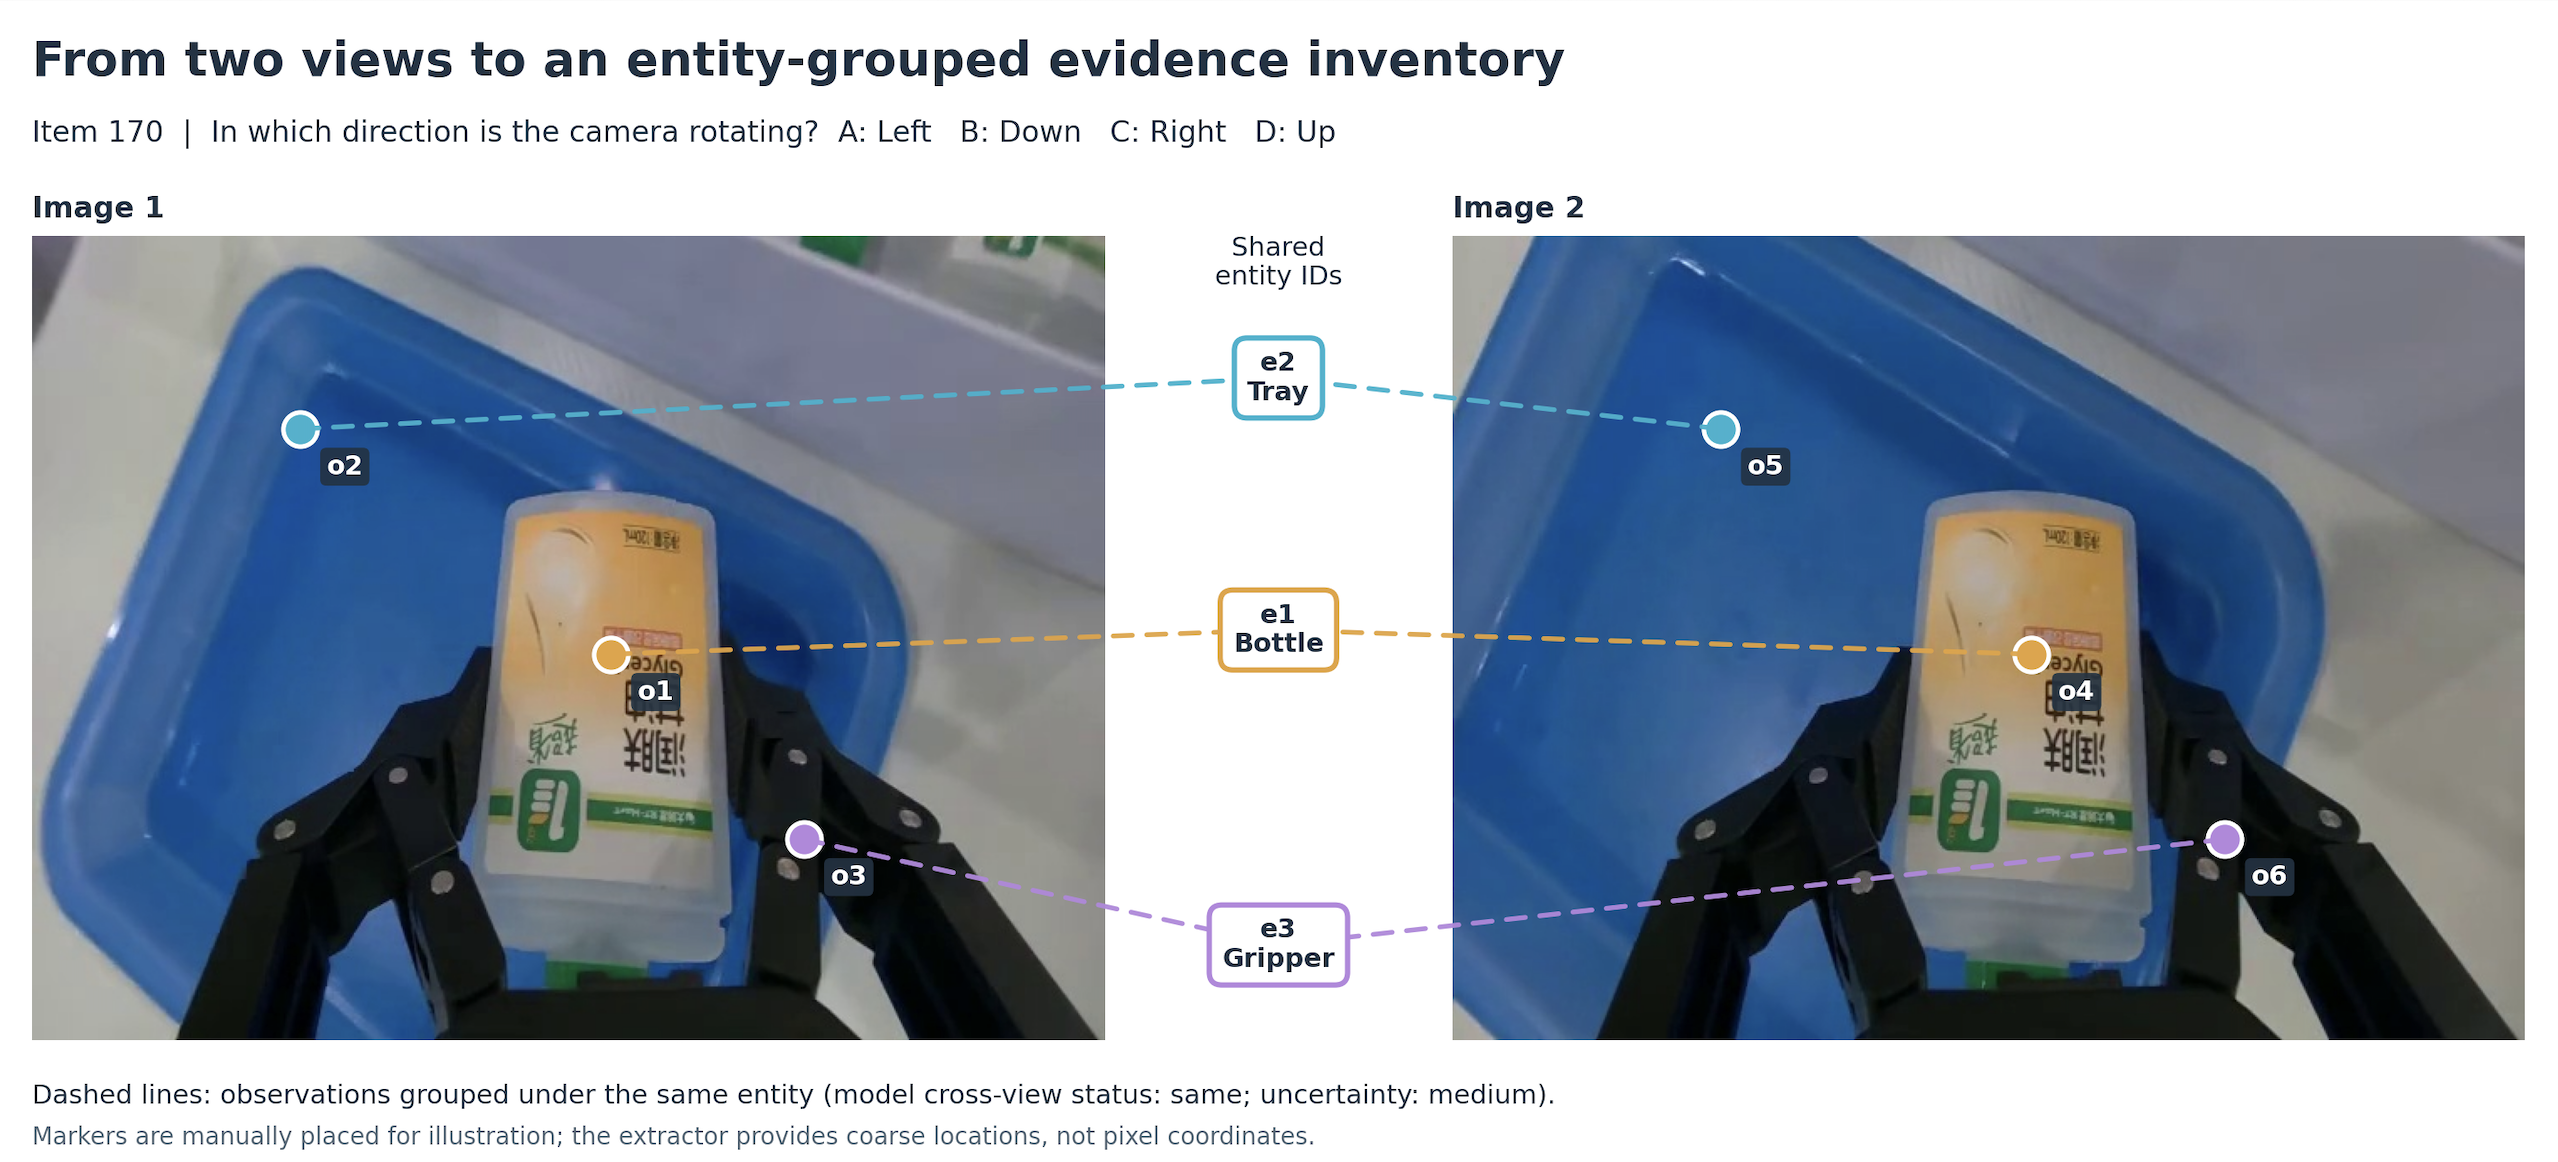
\includegraphics[width=\textwidth]{figures/item170_evidence_organization.png}
  \caption{Entity-grouped evidence on item 170. Colored observation markers
  refer to the saved inventory; dashed lines show membership in shared entity
  IDs, not spatial-relation edges or estimated geometric correspondences.
  Marker positions are manually placed on the original benchmark images:
  the extraction supplies only coarse location labels. Selected JSON fields
  and the corresponding Graph presentation illustrate the shared evidence.
  Graph selects the gold answer B (Down); Raw and Flat select D (Up).
  The inventory itself leaves rotation direction unresolved.}
  \label{fig:worldstate-170}
\end{figure*}
